%% This template can be used to write a paper for
%% Computer Physics Communications using LaTeX.
%% For authors who want to write a computer program description,
%% an example Program Summary is included that only has to be
%% completed and which will give the correct layout in the
%% preprint and the journal.
%% The `elsarticle' style is used and more information on this style
%% can be found at
%% http://www.elsevier.com/wps/find/authorsview.authors/elsarticle.
%%
%%
\documentclass[preprint,review,12pt]{elsarticle}

%% Use the option review to obtain double line spacing
%% \documentclass[preprint,review,12pt]{elsarticle}

%% Use the options 1p,twocolumn; 3p; 3p,twocolumn; 5p; or 5p,twocolumn
%% for a journal layout:
%% \documentclass[final,1p,times]{elsarticle}
%% \documentclass[final,1p,times,twocolumn]{elsarticle}
%% \documentclass[final,3p,times]{elsarticle}
%% \documentclass[final,3p,times,twocolumn]{elsarticle}
%% \documentclass[final,5p,times]{elsarticle}
%% \documentclass[final,5p,times,twocolumn]{elsarticle}

%% if you use PostScript figures in your article
%% use the graphics package for simple commands
\usepackage{graphics}
\usepackage{hyperref}
%% or use the graphicx package for more complicated commands
%% \usepackage{graphicx}
%% or use the epsfig package if you prefer to use the old commands
%% \usepackage{epsfig}

%% The amssymb package provides various useful mathematical symbols
\usepackage{amsmath}
\usepackage{amssymb}
%% The amsthm package provides extended theorem environments
%% \usepackage{amsthm}

%% The lineno packages adds line numbers. Start line numbering with
%% \begin{linenumbers}, end it with \end{linenumbers}. Or switch it on
%% for the whole article with \linenumbers after \end{frontmatter}.
%% \usepackage{lineno}

%% natbib.sty is loaded by default. However, natbib options can be
%% provided with \biboptions{...} command. Following options are
%% valid:

%%   round  -  round parentheses are used (default)
%%   square -  square brackets are used   [option]
%%   curly  -  curly braces are used      {option}
%%   angle  -  angle brackets are used    <option>
%%   semicolon  -  multiple citations separated by semi-colon
%%   colon  - same as semicolon, an earlier confusion
%%   comma  -  separated by comma
%%   numbers-  selects numerical citations
%%   super  -  numerical citations as superscripts
%%   sort   -  sorts multiple citations according to order in ref. list
%%   sort&compress   -  like sort, but also compresses numerical citations
%%   compress - compresses without sorting
%%
%% \biboptions{comma,round}

% \biboptions{}

\usepackage{color}
\usepackage{listings}
\usepackage{textcomp}
\definecolor{listinggray}{gray}{0.9}
\definecolor{lbcolor}{rgb}{0.9,0.9,0.9}
\lstset{
%	backgroundcolor=\color{lbcolor},
        language=Mathematica,
	tabsize=2,
	rulecolor=,
        basicstyle=\scriptsize,
        upquote=true,
%        aboveskip={1.5\baselineskip},
        columns=fixed,
        showstringspaces=false,
        extendedchars=true,
%        breaklines=true,
        prebreak = \raisebox{0ex}[0ex][0ex]{\ensuremath{\hookleftarrow}},
%        frame=single,
        showtabs=false,
        showspaces=false,
        showstringspaces=false,
        identifierstyle=\ttfamily,
        keywordstyle=\color[rgb]{0,0,1},
        commentstyle=\color[rgb]{0.133,0.545,0.133},
        stringstyle=\color[rgb]{0.627,0.126,0.941},
}

\newcommand{\go}{\stackrel{\circ }{\mathfrak{g}}}
\newcommand{\ao}{\stackrel{\circ }{\mathfrak{a}}}
\newcommand{\co}[1]{\stackrel{\circ }{#1}}
\newcommand{\pia}{\pi_{\mathfrak{a}}}
\newcommand{\piab}{\pi_{\mathfrak{a}_{\bot}}}
\newcommand{\gf}{\mathfrak{g}}
\newcommand{\af}{\mathfrak{a}}
\newcommand{\bff}{\mathfrak{b}}
\newcommand{\afb}{\mathfrak{a}_{\bot}}
\newcommand{\hf}{\mathfrak{h}}
\newcommand{\hfg}{\hf_{\gf}}
\newcommand{\hfb}{\mathfrak{h}_{\bot}}
\newcommand{\pf}{\mathfrak{p}}
\newcommand{\aft}{\widetilde{\mathfrak{a}}}

%% This list environment is used for the references in the
%% Program Summary
%%
\newcounter{bla}
\newenvironment{refnummer}{%
\list{[\arabic{bla}]}%
{\usecounter{bla}%
 \setlength{\itemindent}{0pt}%
 \setlength{\topsep}{0pt}%
 \setlength{\itemsep}{0pt}%
 \setlength{\labelsep}{2pt}%
 \setlength{\listparindent}{0pt}%
 \settowidth{\labelwidth}{[9]}%
 \setlength{\leftmargin}{\labelwidth}%
 \addtolength{\leftmargin}{\labelsep}%
 \setlength{\rightmargin}{0pt}}}
 {\endlist}

\journal{Computer Physics Communications}

\begin{document}

\begin{frontmatter}

%% Title, authors and addresses

%% use the tnoteref command within \title for footnotes;
%% use the tnotetext command for the associated footnote;
%% use the fnref command within \author or \address for footnotes;
%% use the fntext command for the associated footnote;
%% use the corref command within \author for corresponding author footnotes;
%% use the cortext command for the associated footnote;
%% use the ead command for the email address,
%% and the form \ead[url] for the home page:
%%
%% \title{Title\tnoteref{label1}}
%% \tnotetext[label1]{}
%% \author{Name\corref{cor1}\fnref{label2}}
%% \ead{email address}
%% \ead[url]{home page}
%% \fntext[label2]{}
%% \cortext[cor1]{}
%% \address{Address\fnref{label3}}
%% \fntext[label3]{}

\title{{\bf Affine.m} -- {\it Mathematica} package for computations in representation theory of finite-dimensional and affine Lie algebras}

%% use optional labels to link authors explicitly to addresses:
%% \author[label1,label2]{<author name>}
%% \address[label1]{<address>}
%% \address[label2]{<address>}

\author[a,b]{Anton Nazarov\corref{author}}
%\author[a,b]{Second Author}
%\author[b]{Third Author}

\cortext[author] {Corresponding author.\\\textit{E-mail address:} antonnaz@gmail.com}
\address[a]{Department of High Energy Physics, Faculty of physics, SPb State University\\ 198904, Sankt-Petersburg, Russia}
\address[b]{Chebyshev Laboratory, Faculty of Mathematics and Mechanics, SPb State University\\ 199178, Saint-Petersburg, Russia}

\begin{abstract}
%% Text of abstract
In this paper we present {\bf Affine.m} -- program for computations in representation theory of finite-dimensional and affine Lie algebras and describe implemented algorithms.  Algorithms are based upon the properties of weights and Weyl symmetry. The most important for us problems are computation of weight multiplicities in irreducible and Verma modules, branching of representations and tensor product decomposition. These problems have numerous applications in physics and we provide some examples of these applications. The program is implemented in popular computer algebra system {\it Mathematica} and works with finite-dimensional and affine Lie algebras. 

% A submitted program is expected to be of benefit to other physicists or physical chemists, or be an exemplar of good programming practice, or illustrate new or novel programming techniques which are of importance to some branch of computational physics or physical chemistry.
%
% Acceptable program descriptions can take different forms. The following Long Write-Up structure is a suggested structure but it is not obligatory. Actual structure will depend on the length of the program, the extent to which the algorithms or software have already been described in literature, and the detail provided in the user manual.

%Your manuscript and figure sources should be submitted through the Elsevier Editorial System (EES) by using the online submission tool at \\
% http://www.ees.elsevier.com/cpc.

%In addition to the manuscript you must supply: the program source code; job control scripts, where applicable; a README file giving the names and a brief description of all the files that make up the package and clear instructions on the installation and execution of the program; sample input and output data for at least one comprehensive test run; and, where appropriate, a user manual. These should be sent, via email as a compressed archive file, to the CPC Program Librarian at cpc@qub.ac.uk.

\end{abstract}

\begin{keyword}
%% keywords here, in the form: keyword \sep keyword
%keyword1; keyword2; keyword3; etc.

Mathematica; Lie algebra; affine Lie algebra; Kac-Moody algebra; root system; weights; irreducible modules, CFT, Integrable systems
\end{keyword}

\end{frontmatter}

%%
%% Start line numbering here if you want
%%
% \linenumbers

% Computer program descriptions should contain the following
% PROGRAM SUMMARY.

{\bf PROGRAM SUMMARY}%/NEW VERSION PROGRAM SUMMARY}
  %Delete as appropriate.

\begin{small}
\noindent
{\em Manuscript Title:}{\bf Affine.m} -- {\it Mathematica} package for computations in representation theory of finite-dimensional and affine Lie algebras                                       \\
{\em Authors:}Anton Nazarov                                                \\
{\em Program Title:}Affine.m                                          \\
{\em Journal Reference:}                                      \\
  %Leave blank, supplied by Elsevier.
{\em Catalogue identifier:}                                   \\
  %Leave blank, supplied by Elsevier.
{\em Licensing provisions:}none                                   \\
  %enter "none" if CPC non-profit use license is sufficient.
{\em Programming language:}Mathematica                                   \\
{\em Computer:}i386-i686, x86\textunderscore 64                                               \\
  %Computer(s) for which program has been designed.
{\em Operating system:} Linux, Windows, MacOS, Solaris                                       \\
  %Operating system(s) for which program has been designed.
{\em RAM:} 5-500 Mb                                              \\
  %RAM in bytes required to execute program with typical data.
%{\em Number of processors used:}                              \\
  %If more than one processor.
%{\em Supplementary material:}                                 \\
  % Fill in if necessary, otherwise leave out.
{\em Keywords:} Mathematica; Lie algebra; affine Lie algebra; Kac-Moody algebra; root system; weights; irreducible modules, CFT, Integrable systems\\
  % Please give some freely chosen keywords that we can use in a
  % cumulative keyword index.
{\em Classification:} 5 Computer Algebra, 4.2 Other algebras and groups                                         \\
  %Classify using CPC Program Library Subject Index, see (
  % http://cpc.cs.qub.ac.uk/subjectIndex/SUBJECT_index.html)
  %e.g. 4.4 Feynman diagrams, 5 Computer Algebra.
%{\em External routines/libraries:}                            \\
  % Fill in if necessary, otherwise leave out.
%{\em Subprograms used:}                                       \\
  %Fill in if necessary, otherwise leave out.
%{\em Catalogue identifier of previous version:}*              \\
  %Only required for a New Version summary, otherwise leave out.
%{\em Journal reference of previous version:}*                  \\
  %Only required for a New Version summary, otherwise leave out.
%{\em Does the new version supersede the previous version?:}*   \\
  %Only required for a New Version summary, otherwise leave out.
{\em Nature of problem:}\\
  %Describe the nature of the problem here.
Representation theory of finite-dimensional Lie algebras has many applications in different branches of physics, including elementary particle physics, molecular physics, nuclear physics. Representations of affine Lie algebras appear in string theories and two-dimensional conformal field theory used for the description of critical phenomena in two-dimensional systems. Also Lie symmetries play major role in study of quantum integrable systems.
   \\
{\em Solution method:}\\
  %Describe the method solution here.
We work with weights and roots of finite-dimensional and affine Lie algebras and use Weyl symmetry extensively. Central problems which are the computations of weight multiplicities, branching and fusion coefficients are solved using one general recurrent algorithm based on generalization of Weyl character formula. We also offer alternative implementation based on Freudenthal multiplicity formula which can be faster in some cases.
   \\
%{\em Reasons for the new version:}*\\
  %Only required for a New Version summary, otherwise leave out.
%   \\
%{\em Summary of revisions:}*\\
  %Only required for a New Version summary, otherwise leave out.
%   \\
{\em Restrictions:}\\
  %Describe any restrictions on the complexity of the problem here.
Computational complexity grows fast  with the rank of algebra, so computations for algebra of rank greater than 8 are non practical.
   \\
{\em Unusual features:}\\
  %Describe any unusual features of the program/problem here.
We offer the possibility to use traditional mathematical notation for objects in representation theory of Lie algebras in computations if {\bf Affine.m} is used in {\it Mathematica} notebook interface.
   \\
%{\em Additional comments:}\\
  %Provide any additional comments here.
%   \\
{\em Running time:}\\
  %Give an indication of the typical running time here.
From seconds to days depending on rank of algebra and complexity of representations.
   \\

% \begin{thebibliography}{0}
% \bibitem{1}Reference 1         % This list should only contain those items referenced in the
% \bibitem{2}Reference 2         % Program Summary section.
% \bibitem{3}Reference 3         % Type references in text as [1], [2], etc.
%                                % This list is different from the bibliography at the end of
%                                % the Long Write-Up.
% \end{thebibliography}
% * Items marked with an asterisk are only required for new versions
% of programs previously published in the CPC Program Library.\\
\end{small}


%% main text
\section{Introduction}
\label{intro}

Representation theory of Lie algebras is of central importance for different areas of physics and mathematics. In physics Lie algebras are used for the description of symmetries of quantum and classical systems. Computational methods in representation theory have a long history \cite{belinfante1989survey}, there exist numerous software packages for computations related to Lie algebras \cite{simplie}, \cite{vanleeuwen1994lsp}, \cite{stembridge1995mps,coxweyl}, \cite{fischbacher2002ilp}, \cite{Fuchs:1996dd}.

Most popular programs \cite{simplie}, \cite{vanleeuwen1994lsp}, \cite{fischbacher2002ilp}, \cite{coxweyl} are created to study representation theory of simple finite-dimensional Lie algebras. The main computational problems are the following:
\begin{enumerate}
\item Construction of root system which determine the properties of Lie algebra including its commutation relations.
\item Weyl group traversal which is important due to Weyl symmetry of root system and characters of representations.
\item Calculation of weight multiplicities, branching and fusion coefficients, which are essential for construction and study of representations.
\end{enumerate}
There are well-known algorithms for these tasks \cite{moody1982fast}, \cite{stembridge2001computational}, \cite{belinfante1989survey}, \cite{casselman1994machine}.
The third problem is most computation-intensive. There are two different recurrent algorithms which are based on Weyl character formula and Freudenthal multiplicity formula. In this paper we analyze them.

Infinite-dimensional Lie algebras also have growing number of applications in physics for example in conformal field theory and study of  integrable systems. But infinite-dimensional algebras are much harder to study and number of available computer programs is much smaller.

Affine Lie algebras \cite{kac1990idl} constitute important and tractable class of infinite-dimensional Lie algebras. They are constructed as the central extensions of loop algebras of (semi-simple) finite-dimensional Lie algebras and appear naturally in the study of Wess-Zumino-Witten and coset models of conformal field theory \cite{Walton:1999xc}, \cite{difrancesco1997cft}, \cite{Goddard198588}, \cite{Dunbar:1992gh}.

The structure of affine Lie algebras allows to extend computational algorithms created for finite-dimensional Lie algebras  \cite{Fuchs:1996dd}, \cite{gannon2001algorithms}, \cite{kass1990ala}. The book \cite{kass1990ala} with the tables of multiplicities and other computed characteristics of affine Lie algebras and representations was published in 1990. But we are not aware of software packages for popular computer algebra systems which can be used to extend these results.
We address this issue and present {\bf Affine.m} -- {\it Mathematica} package for computations in representation theory of affine and finite-dimensional Lie algebras.  We describe the features and limitations of the package in present paper.  We also provide representation-theoretical background of implemented algorithms and present some examples of computations relevant to physics.

The paper is started with an overview of Lie algebras and their representation theory (Sec. \ref{sec:theor-backgr}). Then we describe datastructures of {\bf Affine.m} used to present different objects related to Lie algebras and representations (Sec. \ref{sec:core-datastructures}) and discuss implemented algorithms (Sec. \ref{sec:comp-algor}). Next section consists of physically interesting examples (Sec. \ref{sec:examples}). The paper is concluded with the discussion of possible extensions and refinements (Sec. \ref{sec:conclusion}).

\section{Theoretical background}
\label{sec:theor-backgr}

In this section we remind necessary definitions and present formulae used in computations. 

\subsection{Lie algebras of finite and affine types}
\label{sec:lie-algebras-finite}

{\it Lie algebra} $\gf$ is a vector space with bilinear operation $[\cdot,\cdot]:\gf\otimes\gf\to \gf$, which is called {\it commutator}. If we choose the basis $X_{i}$ in $\gf$ we can specify commutation relations by the {\it structure constants} $C_{ijk}$:
\begin{equation}
  \label{eq:1}
  [X^{i},X^{j}]=\sum_{k} C^{ij}_{k} X^{k}
\end{equation}
Lie algebra is {\it simple} if it contains no non-trivial ideals with respect to commutator. {\it Semisimple} Lie algebra is a direct sum of simple Lie algebras. In present paper we treat simple and semisimple Lie algebras. 

Maximal commutative subalgebra ({\it Cartan subalgebra}) of $\gf$ is denoted by $\hfg$.
We denote the elements of basis of $\hfg$ by $H^{i}$.

Killing form on $\gf$ gives a non-degenerate bilinear form $(\cdot,\cdot)$ on $\hfg$ which can be used to identify $\hfg$ with the subspace of the dual space $\hfg^{*}$ of linear functionals on $\hfg$. {\it Weights} are the elements of $\hfg^{*}$ and are denoted by Greek letters $\mu,\nu, \omega, \lambda\dots$

Special choice of basis gives compact description of commutation relations (\ref{eq:1}). This basis can be encoded by the root system which is discussed in Section \ref{sec:weights-roots} (See also \cite{humphreys1997introduction,humphreys1992reflection}).

{\it Loop algebra} $L\gf=\gf\otimes \mathbb{C}[t,t^{-1}]$, corresponding to semisimple Lie algebra $\gf$, has commutation relations
\begin{equation}
  \label{eq:6}
  [X^{i}t^{n},X^{j}t^{m}]=t^{n_+m}\sum_{k}C^{ij}_{k}X^{k}
\end{equation}
Central extension leads to the appearance of additional term
\begin{equation}
  \label{eq:7}
   [X^{i}t^{n}+\alpha c,X^{j}t^{m}+\beta c]=t^{n+m}\sum_{k}C^{ij}_{k}X^{k}+(X^{i},X^{j})n\delta_{n+m,0}c
\end{equation}
This algebra $\hat\gf=\gf\otimes\mathbb{C}[t,t^{-1}]\oplus\mathbb{C}c$ is called {\it affine Lie algebra} \cite{kac1990idl}, \cite{wakimoto2001idl,wakimoto2001lectures}, \cite{kass1990ala}.

Sometimes we denote affine Lie algebra by $\gf$ then corresponding finite-dimensional Lie algebra is denoted by $\go$.

\subsection{Modules, weights and roots}
\label{sec:weights-roots}

Let $\gf$ be finite-dimensional or affine Lie algebra.

Then $\gf$-module is a vector space $V$ together with a bilinear map $\gf \times V\to V$ such that
\begin{equation}
  \label{eq:2}
  [x,y]\cdot v = x\cdot(y\cdot v) - y\cdot(x\cdot v), \quad \mbox{for}\; x,y\in \gf, v\in V
\end{equation}
Representation of algebra $\gf$ on a vector space $V$ is the homomorphism $\gf\to gl(V)$ from $\gf$ to Lie algebra of endomorphisms on vector space $V$ with the commutator as the bracket.

For an arbitrary representation it is possible to diagonalize the operators corresponding to Cartan generators $H^{i}$ simultaneously by special choice of basis $\{v_{j}\}$ in $V$:
\begin{equation}
  \label{eq:3}
  H^{i}\cdot v_{j}=\nu_{j}^{i}v_{j}
\end{equation}
Eigenvalues $\nu^{i}_{j}$ of Cartan generators on element of basis $v_{j}$ determine weight $\nu_{j}\in \hfg^{*}$ such that $\nu_{j}(H^{i})=\nu_{j}^{i}$. Vector $v\in V$ is called weight vector of weight $\lambda$ if $H v=\lambda_{j}(H)v,\; \forall H\in \hf$ , weight subspace consists of all weight vectors $V_{\lambda}=\{v\in V: H v=\lambda_{j}(H)v,\; \forall H\in \hf\}$. Weight multiplicity $m_{\lambda}=\mathrm{mult}(\lambda)=\mathrm{dim} V_{\lambda}$ is the dimension of weight subspace.

The structure of module is determined by the set of weights since the action of generators $E^{\alpha}$ on a weight vectors is
\begin{equation}
  \label{eq:5}
  E^{\alpha}\cdot v_{\lambda} \propto v_{\lambda+\alpha}
\end{equation}
Module structure can be encoded by the formal character of module
\begin{equation}
  \label{eq:10}
  \mathrm{ch}V=\sum_{\lambda}m_{\lambda} e^{\lambda}
\end{equation}
Character  $\mathrm{ch}V\in \mathcal{E}$ is an element of algebra $\mathcal{E}$ generated by formal exponents of weights.
Character can be specialized by taking its value on some element $\xi$ of $\hf$:

Lie algebra is its own module. The action of generators is called adjoint and it is given by the bracket $ad_{X} Y=[X,Y]$. 
{\it Roots} are weights of adjoint representation of $\gf$. They encode the commutation relations of algebra in the following way. Denote by $\Delta$ the set of roots. For each $\alpha\in \Delta$ there exist a root $-\alpha\in \Delta$ and generators $E^{\alpha}, E^{-\alpha}$ such that
\begin{align}
  \label{eq:4}
  &  [H^{i},E^{\alpha}]=\alpha^{i}E^{\alpha} \\
  &\left[E^{\alpha},E^{\beta}\right]=
  \begin{cases}
    N_{\alpha,\beta} E^{\alpha+\beta}, & \mbox{if}\; \alpha+\beta\in \Delta\\
    \frac{2}{(\alpha,\alpha)} \sum_{i}\alpha^{i} H^{i},&  \mbox{if}\; \alpha=-\beta\\
    0,&\mbox{otherwise}
  \end{cases}
\end{align}

Given a root system $\Delta$ we can choose a set of positive roots. This is a subset  $\Delta^{+}\subset \Delta$ such that for each root $\alpha\in\Delta$ exactly one of the roots $\alpha, -\alpha$ is contained in $\Delta^{+}$ and for any two distinct positive roots $\alpha, \beta\in \Delta^{+}$ such that $\alpha+\beta\in \Delta$ their sum is also positive $\alpha+\beta\in\Delta^{+}$.
Elements of $-\Delta^{+}$ are called negative roots.

A positive root is {\it simple} if it cannot be written as the sum of positive roots. The set of simple roots $\Phi=\left\{\alpha_{i}\right\}$ is a basis of $\hfg$ and each root can be written as $\alpha=\sum_{i}n_{i}\alpha_{i}$ with all $n_{i}$ non-negative or non-positive. In case of finite-dimensional Lie algebra $\gf$ simple roots are numbered from 1 to rank of the algebra $i=1,\dots,r,\quad r=\mathrm{rank}(\gf)$. By numbering simple roots with an index $i$ we introduce an ordering on the root system $\Delta$. Highest root with respect to this ordering is denoted by  $\theta=\sum_{i=1,\dots,r} a_i \alpha_i$, coefficients $a_i$ are called {\it marks}. It is also highest weight (See section \ref{sec:high-weight-modul}) of adjoint module. {\it Comarcs} are equal to $a_i^{\vee}=\frac{(\alpha_i,\alpha_i)}{2} a_i$.

Although the full set of roots $\Delta$ is infinite for affine Lie algebra $\hat\gf$ the set of simple roots $\Phi$ is finite and its elements are denoted by $\alpha_{0},\dots \alpha_{r}$ where $r=\mathrm{rank}(\gf)$. The roots $\alpha_1,\dots, \alpha_r$ are the roots of the underlying finite-dimensional Lie algebra $\go$. The root $\alpha_0=\delta-\theta$ is the difference of {\it imaginary root} $\delta$ and $\theta$ -- highest root of the algebra $\go$.
Note that root multiplicity $\mathrm{mult}(\alpha)$ for affine Lie algebra can be greater than one.

Sub-algebra  $\bff_{+}\subset \gf$ spanned by the generators $H^{i}, E^{\alpha}$ for $\alpha\in \Delta^{+}$ positive is called Borel sub-algebra.

{\it Parabolic subalgebra}  $\pf_{I}\supset \bff_{+}$ contains Borel subalgebra and is  generated by some subset of simple roots $\{\alpha_{j}:j\in I, I\subset \{1\dots r\}\}$. It is spanned by the subset of generators $\{H^{i}\}\cup \{E^{\alpha}:\alpha\in \Delta^{+}\}\cup \{E^{-\alpha}: \alpha\in\Delta^{+}, \alpha=\sum_{j\in I} n_{j} \alpha_{j}\}$.

{\it Regular subalgebra} $\af\subset\gf$ is determined by the root system $\Delta_{\af}$ with the set of simple roots $\{\beta_{i}, i=1,\dots,r_{\af}\}$ which is a subset of set of simple roots $\{\alpha_{1},\dots,\alpha_{r}\}\cup \{\Theta\}$ with the addition of highest root.

The Weyl group $W_{\gf}$ is generated by reflections $\{s_{i}:\hfg^{*}\to\hfg^{*}\}$ corresponding to simple roots $\{\alpha_{i}\}$:
\begin{equation}
  \label{eq:8}
  s_{i}\cdot\lambda=\lambda-\frac{2(\alpha_{i},\lambda)}{(\alpha_{i},\alpha_{i})}\alpha_{i}
\end{equation}
Root system and characters of representation are invariant with respect to the action of Weyl group. Root system can be reconstructed from the set of simple roots with the action of Weyl group.

Weyl groups are finite for finite-dimensional Lie algebras and finitely-generated for affine Lie algebras.

Consider an action of element $s_{0}s_{i}s_{0}$ of Weyl group of affine Lie algebra  $\hat\gf$. Using the definition \eqref{eq:8} it is easy to see that $s_{0}s_{i}s_{0}\cdot \lambda=\lambda+\alpha_{i}$, so Weyl group can be presented as semidirect product of Weyl group $W_{\gf}$ of $\gf$ and translations by the roots of $\hat \gf$. Weyl group element can be presented as the product of elementary reflections in multiple ways. Number of elementary reflections in shortest sequence representing element $w\in W_{\gf}$ is called {\it length} of $w$ and denoted $l(w)$. We also use the notation $\epsilon(w)=(-1)^{l(w)}$ for parity of number of Weyl reflections generating $w$. 

Fundamental domain $\bar{C}$ for the action of Weyl group $W_{\gf}$ on $\hfg^{*}$ is determined by the requirement $\xi\in \bar{C}\Leftrightarrow (\xi,\alpha_{i})\geq 0$ for all simple roots $\alpha_{i}$. It is called {\it main Weyl chamber}. 

The Cartan matrix $A$ is defined by products of simple roots
\begin{equation}
  \label{eq:9}
  A_{ij}=\frac{2(\alpha_{i},\alpha_{j})}{(\alpha_{j},\alpha_{j})}
\end{equation}
and can be used for compact description of Lie algebra commutation relations in Chevalley basis \cite{humphreys1997introduction}, \cite{fulton1991representation}, \cite{bourbaki2002lie}.

The form \eqref{eq:9} induces the basis dual  to the simple
roots basis. It is called the fundamental weights basis. We denote
its elements by $\omega_i$:
\begin{equation}
  \label{eq:20}
  \langle\omega_i,\alpha_j\rangle=\frac{2(\omega_{i},\alpha_{j})}{(\alpha_{j},\alpha_{j})}=\delta_{ij}
\end{equation}
For finite-dimensional Lie algebra there are $r$ fundamental weights, $i=1,\dots, r$. For affine Lie algebra we have additional fundamental weight $\omega_0=\lambda$, $(\lambda,\delta)=1, \; (\lambda,\lambda)=(\delta,\delta)=0$. Other fundamental weights are equal to $\omega_i=a_i^v \lambda_0 +\co{\omega_i}$, where $\co{\omega_i}$ is the fundamental weight of finite-dimensional Lie algebra $\go$.

We need to introduce Weyl vector denoted by $\rho=\sum_{i} \omega_{i}$. It is of importance for the construction of algebra modules.

\subsection{Highest weight modules}
\label{sec:high-weight-modul}

We consider finitely-generated $\gf$-modules $V$ such that $V=\bigoplus_{\xi\in \hfg^{*}} V_{\xi}$, where each $V_{\xi}$ is finite-dimensional and there exists finite set of weights $\lambda_{1},\dots \lambda_{s}$ which generates weight system of $V$, i.e. if $\mathrm{dim}V_{\xi}\neq 0$ then $\xi=\lambda_{i}-\sum_{k=1,\dots, r} n_{k}\alpha_{k}$ where $n_{k}\in \mathbb{Z}_{+}$ (See \cite{humphreys2008representations}, \cite{carter2005lie}).

Highest weight module $V^{\mu}$ contains one highest weight $\mu$, all other weights are obtained by the subtraction of linear combination of simple roots $\lambda=\mu-n_{1}\alpha_{1}-\dots-n_{r}\alpha_{r},\; n_{k}\in \mathbb{Z}_{+}$.

The most simple type of highest weight modules is the Verma module
$M^{\mu}$ who's space can be defined as the space
\begin{equation}
  \label{eq:17}
  M^{\mu}=U(\gf)\underset{U(\bff_{+})}{\otimes} D^{\mu}(\bff_{+}),
\end{equation}
with respect to the multiplication in $U(\gf)$,
where $\underset{U(\bff_{+})}{\otimes}$ means that the action of elements of $U(\bff_{+})$ ``falls through'' the left part of tensor product onto the right part. Here $\bff_{+}$ is Borel sub-algebra, $D^{\mu}(\bff_{+})$ is a representation of $\bff_{+}$ such that $D(E^{\alpha})=0,\; D(H)=\mu(H)$ for any positive root $\alpha$.
Elements of $\gf$ act from the left and we should commute all the elements of $\bff_{+}$ to the right, so that they can act on the space $D_{\lambda}(\bff_{+})$.

Weight multiplicities in Verma module can be found from the Weyl
character formula
\begin{equation}
  \label{eq:11}
  \mathrm{ch} M^{\mu}=\frac{e^{\mu}}{\prod_{\alpha\in \Delta^{+}} \left( 1-e^{-\alpha}\right)^{\mathrm{mult}(\alpha)}}=\frac{e^{\mu}}{\sum_{w\in W} \epsilon(w) e^{w\rho-\rho}}
\end{equation}
Here we have used the Weyl denominator identity
\begin{equation}
  \label{eq:12}
  R:=\prod_{\alpha\in \Delta^{+}} \left( 1-e^{-\alpha}\right)^{\mathrm{mult}(\alpha)}=\sum_{w\in W} \epsilon(w) e^{w\rho-\rho},
\end{equation}
and $\epsilon \left( w\right) :=\det \left( w\right)$ is equal to 
the parity of number of Weyl reflections generating $w$.

Verma module $M^{\mu}$ has the unique maximal submodule and the
unique nontrivial simple quotient $L^{\mu}$ which is an
irreducible highest weight module. Weyl character formula for
irreducible highest weight modules is
\begin{equation}
  \label{eq:13}
  \mathrm{ch} L^{\mu}=\frac{\sum_{w\in W} \epsilon(w) e^{w(\mu+\rho)-\rho}}{\sum_{w\in W}\epsilon(w) e^{w\rho-\rho}}=\sum_{w\in W} \epsilon(w)\; \mathrm{ch} M^{w(\mu+\rho)-\rho}
\end{equation}
Thus the character of an irreducible highest weight module can be
seen as the combination of characters of Verma modules. ( This
fact is a consequence of the Bernstein-Gelfand-Gelfand resolution
(\cite{bernstein1976category,bernstein1971structure}, see also
\cite{humphreys2008representations}).)

Construction of generalized Verma modules is analogous to (\ref{eq:17}), but representation of Borel subalgebra is substituted by the representation of parabolic subalgebra $\pf_{I}\supset \bff_{+}$ generated by some subset $\{\alpha_{I}\}$ of simple roots $I\subset \{1,\dots, r\}$:
\begin{equation*}
M_{I}^{\mu}=U\left( \gf\right)\otimes _{U\left( \pf_{I}\right) }L_{\pf_{I}}^{\mu}.
\end{equation*}
Denote a formal element $R_{I}:=\prod_{\alpha \in \Delta
^{+}\setminus \Delta _{\pf_{I}}^{+}}\left( 1-e^{-\alpha }\right)
^{\mathrm{mult}(\alpha )}$. Then the character of generalized
Verma module can be written as
\begin{equation}
  \label{eq:18}
  \mathrm{ch}M_{I}^{\mu}=\frac{1}{R_{I}}\mathrm{ch}L_{\pf_{I}}^{\mu }.
\end{equation}


%% Define external border of irreducible representation here

We can use Weyl character formula to obtain recurrent relation on weight multiplicities which can be used for calculations \cite{il2010folded,kulish4sfa}:
\begin{equation}
\label{eq:14}
m_{\xi }=-\sum_{w\in W\setminus e}\epsilon (w)m_{\xi
-\left( w(\rho )-\rho \right) }+\sum_{w\in W}\epsilon
(w)\delta _{\left( w(\mu +\rho )-\rho \right) ,\xi }.
\end{equation}

Other recurrent formula can be obtained from the study of Casimir
elements action on irreducible highest weight modules
\cite{humphreys1997introduction}:
\begin{equation}
  \label{eq:15}
  m_{\lambda}=\frac{2}{(\mu+\rho)^{2}-(\lambda+\rho)^{2}}\sum_{\alpha\in \Delta^{+}}\sum_{k\geq 1} (\lambda+k\alpha,\alpha)m_{\lambda+k\alpha}.
\end{equation}
It is called the Freudenthal multiplicity formula.

Now consider an algebra $\gf$ and a reductive subalgebra
$\af\subset \gf$. Simple roots $\beta_{i}$ of the subalgebra $\af$
can be presented as linear combinations of algebra roots
$\alpha_{j}$: $\beta_{i}=\sum_{j=1,\dots,r_{\gf}}k_{j}
\alpha_{j},\ j=1,\dots,r_{\af}$.

Each $\gf$-module is also an $\af$-module, although
$L^{\mu}_{\gf}$ is not irreducible as $\af$-module. It can be
decomposed into the sum of irreducible $\af$-modules:
\begin{equation}
  \label{eq:16}
  L^{\mu}_{\gf}=\bigoplus_{\nu}b^{\mu}_{\nu}L^{\nu}_{\af}
\end{equation}
Coefficients in this decomposition are called the branching
coefficients. 

Before we proceed to recurrent relation for branching coefficients we need several definitions.

For a subalgebra $\af\subset \gf$ we introduce a subalgebra
$\afb$. Consider the root subspace $\hf_{\perp \af}^{\ast }$
orthogonal to $\af$,
\begin{equation*}
\hf_{\perp \af}^{\ast }:=\left\{ \eta \in \hf^{\ast }|\forall
h\in \hf_{\af};\eta \left( h\right) =0\right\} ,
\end{equation*}
and the roots (correspondingly -- positive roots) of $\gf$ orthogonal
to $\af$,
\begin{eqnarray}
\Delta _{\afb} &:&=\left\{ \beta \in \Delta _{\gf}|\forall
h\in \hf_{\af};\beta \left( h\right) =0\right\} ,
\label{delta a ort} \\
\Delta _{\afb}^{+} &:&=\left\{ \beta ^{+}\in \Delta _{\gf%
}^{+}|\forall h\in \hf_{\af};\beta ^{+}\left( h\right) =0\right\} .
\notag
\end{eqnarray}
Let $W_{\afb}$ be the subgroup of $W$ generated by the
reflections $w_{\beta }$ with the roots $\beta \in \Delta _{\af_{\perp
}}^{+}$. The subsystem $\Delta _{\afb}$ determines the
subalgebra $\afb$ with the Cartan subalgebra $\hf_{\af%
_{\perp }}$.

For $\af$ and $\afb$ consider the
corresponding Weyl vectors, $\rho _{\af}$ and $\rho _{\af_{\perp
}} $.

Compose the so called ''defects'' $\mathcal{D}_{\af}$ and $\mathcal{%
D}_{\afb}$ of the injection:
\begin{equation}
\mathcal{D}_{\af}:=\rho _{\af}-\pi _{\af}\rho , \qquad
\mathcal{D}_{\afb}:=\rho _{\afb}-\pi _{\af%
_{\perp }}\rho .  \label{defect-ort}
\end{equation}

For $\mu \in P^{+}$ consider the linked weights $\left\{ \left(
w(\mu +\rho )-\rho \right) |w\in W\right\} $ and their projections
to
$h_{\afb}^{\ast }$ additionally shifted by the defect $-%
\mathcal{D}_{\afb}$:
\begin{equation*}
\mu _{\afb}\left( w\right) :=\pi _{\afb}\left[
w(\mu +\rho )-\rho \right] -\mathcal{D}_{\afb},\quad w\in W.
\end{equation*}
Among the weights $\left\{ \mu _{\af_{\perp
}}\left( w\right) |w\in W\right\} $ one can always choose those located in
the fundamental chamber $\overline{C_{\afb}}$. Let $U$ be the
set of representatives $u$ for the classes $W/W_{\afb}$ such
that

\begin{equation}
U:=\left\{ u\in W|\quad \mu _{\afb}\left( u\right) \in
\overline{C_{\afb}}\right\} \quad .  \label{U-def}
\end{equation}
Thus we can form the subsets:
\begin{equation}
\mu _{\widetilde{\mathfrak{a}}}\left( u\right) :=\pi _{\widetilde{%
\mathfrak{a}}}\left[ u(\mu +\rho )-\rho \right] +\mathcal{D}_{\af%
_{\perp }},\quad u\in U,  \label{mu-a}
\end{equation}
and
\begin{equation}
\mu _{\afb}\left( u\right) :=\pi _{\afb}\left[
u(\mu +\rho )-\rho \right] -\mathcal{D}_{\afb},\quad u\in U.
\label{mu-a-tilda}
\end{equation}

Notice that the subalgebra $\mathfrak{a}_{\bot}$ is regular by definition
since it is built on a subset of roots of the algebra $\mathfrak{g}$.

Denote by  $k_{\xi }^{\left( \mu \right) }$ signed branching coefficients. If $\xi\in \bar C_{\af}$ is in main Weyl chamber $k_{\xi}^{(\mu)}=b^{(\mu)}_{\xi}$ otherwise $k_{\xi}^{(\mu)}=\epsilon(w) b^{(\mu)}_{w (\xi+\rho_{\af})-\rho_{\af}}$ where $w\in W_{\af}$ is such that $w (\xi+\rho_{\af})-\rho_{\af}\in W_{\af}$. 

Now we can use the Weyl character formula to write a
recurrent relation \cite{2010arXiv1007.0318L} for signed branching
coefficients $k_{\xi }^{\left( \mu \right) }$ corresponding to an
injection $\af\hookrightarrow \gf$:
\begin{equation}
\begin{array}{c}
k_{\xi }^{\left( \mu \right) }=-\frac{1}{s\left( \gamma _{0}\right) }\left(
\sum_{u\in U}\epsilon (u)\;\dim \left( L_{\afb}^{\mu _{\af%
_{\perp }}\left( u\right) }\right) \delta _{\xi -\gamma _{0},\pi _{%
\widetilde{\af}}(u(\mu +\rho )-\rho )}+\right.  \\
\left. +\sum_{\gamma \in \Gamma _{\widetilde{\af}\rightarrow \gf%
}}s\left( \gamma +\gamma _{0}\right) k_{\xi +\gamma }^{\left( \mu \right)
}\right) .
\end{array}
\label{recurrent-rel}
\end{equation}
The recursion is goverened by the set $\Gamma _{\widetilde{\af}\rightarrow \gf}$ called the injection fan. The latter is defined by the
carrier set $\left\{ \xi \right\} _{\af\rightarrow \gf}$ for the
coefficient function $s(\xi )$
\begin{equation*}
\left\{ \xi \right\} _{\widetilde{\af}\rightarrow \gf}:=\left\{
\xi \in P_{\widetilde{\af}}|s(\xi )\neq 0\right\}
\end{equation*}
appearing in the expansion
\begin{equation}
\prod_{\alpha \in \Delta ^{+}\setminus \Delta _{\bot }^{+}}\left( 1-e^{-\pi
_{\widetilde{\af}}\alpha }\right) ^{\mathrm{mult}(\alpha )-\mathrm{mult}%
_{\af}(\pi _{\widetilde{\af}}\alpha )}=-\sum_{\gamma \in P_{%
\widetilde{\af}}}s(\gamma )e^{-\gamma };\quad
\end{equation}
The weights in $\left\{ \xi \right\} _{\widetilde{\af}\rightarrow \gf}$ are to be shifted by $\gamma _{0}$ -- the lowest vector in $\left\{ \xi
\right\} $ -- and the zero element is to be eliminated:
\begin{equation}
\Gamma _{\widetilde{\af}\rightarrow \gf}=\left\{ \xi -\gamma
_{0}|\xi \in \left\{ \xi \right\} \right\} \setminus \left\{ 0\right\} .
\end{equation}
The formula (\ref{eq:14}) is a particular case of recurrent relation for branching coefficients (\ref{recurrent-rel}) in the case of Cartan subalgebra $\af=\hfg$.

If the root system of $\afb$ is generated by some subset of $\gf$
simple roots $\alpha_{1},\dots,\alpha_{r}$ then the recurrent
relation (\ref{recurrent-rel}) is connected with the generalized
Bernstein-Bernstein-Gelfand resolution for parabolic Verma modules
\cite{2011arXiv1102.1702L}.

Another particular case of this formula is connected with tensor
product decomposition. Consider the tensor product of two
irreducible $\gf$-modules $L^{\mu}\otimes L^{\nu}$. It is also a
$\gf$-module but not irreducible in general. So
\begin{equation}
  \label{eq:19}
  L^{\mu}\otimes L^{\nu}=\bigoplus_{\gamma} f^{\mu\nu}_{\gamma}L^{\gamma}
\end{equation}
The coefficients $f^{\mu\nu}_{\gamma}$ are called fusion
coefficients. The problem of computation of fusion coefficients is
equivalent to branching problem for the diagonal subalgebra
$\gf\subset \gf\otimes \gf$ (see \cite{LyakhovskyPostnova2011}).

In the case of affine Lie algebras $\gf, \af$  the multiplicities
$m_{\nu}$ and the corresponding branching coefficients $b_{\nu}$
can be regarded as the coefficients in power series decomposition
of string and branching functions correspondingly:
\begin{align}
  \label{eq:21}
  &\sigma_{\nu}(q)=\sum_{n=0}^{\infty} m_{\nu-n\delta} q^n, \quad \nu=\sum_j c_j \omega_j,\quad c_j\geq 0\\
  & b_{\nu}(q)=\sum_{n=0}^{\infty} b_{\nu-n\delta} q^n,\quad  \nu=\sum_j c_j \omega_j, \quad c_j\geq 0
\end{align}

String and branching functions have  modular and analytic properties which are important for conformal field theory, especially in  coset models and the study of CFT on higher genus surfaces \cite{kac1988modular}, \cite{difrancesco1997cft}, \cite{Walton:1999xc}, \cite{walton1989conformal}.

\section{Core datastructures}
\label{sec:core-datastructures} Having introduced necessary
mathematical objects, problems and relations we now describe the
related datastructures of {\bf Affine.m}. Although {\it
Mathematica} is untyped language it is possible to create
structured objects and do type checks with patterns
\cite{shifrinmathematica}, \cite{maeder2000computer}.
\subsection{Weights}
\label{sec:weights}

Weights are represented  by two data-structures: \lstinline{finiteWeight} for finite-dimensional Lie algebras and \lstinline{affineWeight}  for affine.

Internally the finite weight is a \lstinline{List} with the
\lstinline{Head} \lstinline{finiteWeight}, its components are the
coordinates of the weight in the orthogonal basis of
\cite{bourbaki2002lie}.

Affine weight is an extension of a finite weight by supplying it
with level and grade coordinates. There is a set of functions
defined for finite and affine weights. The complete list can be
found in package online help. The most important
are the definitions of addition, multiplication by number and
scalar product (bilinear form) for weights. These definitions
allow to use traditional notation when working with {\bf
Affine.m}:
\begin{lstlisting}
  w=makeFiniteWeight[{1,0,3}];
  v=makeFiniteWeight[{3,2,1}];
  2*w+v==makeFiniteWeight[{5,2,7}]
  w.v==6
\end{lstlisting}

The use of orthogonal basis in the internal structure of weights allows us to work with weights without complete specification of root system which is useful for study of branching, since roots of the subalgebra can be specified by hand.

\subsection{Root systems}
\label{sec:root-systems}

To specify an algebra of finite or affine type it is enough to fix
its root system. Root systems are represented by two datatypes
\lstinline{finiteRootSystem} and \lstinline{affineRootSystem}. The
latter is an extension of the former. We offer several different
constructors for these datastructures. It is possible to specify
the set of simple roots explicitly, for example to study the
subalgebra $B_2\subset B_4$ we can use the definition
\begin{lstlisting}
  b2b4=makeFiniteRootSystem[ { {1,-1,0,0}, {0,1,0,0} } ]
\end{lstlisting}
There are constructors for root systems of simple finite-dimensional Lie algebras:
\begin{lstlisting}
  b2=makeSimpleRootSystem[B,2]
\end{lstlisting}
We use typographic features of {\it Mathematica} frontend to offer traditional mathematical notation for simple Lie algebras:


\begin{lstlisting}[mathescape=true]
  $B_2$ == makeFiniteRootSystem[ { {1, -1}, {0, 1} }]
\end{lstlisting}

Non-twisted affine root systems can be created as affine extensions of finte root systems, e.g.
\begin{lstlisting}
  b2affine = makeAffineExtension[b2]
\end{lstlisting}
In notebook interface this can be written simply as $\hat{B}_2$.

Semisimple Lie algebras can be created as sums of simple:
\begin{lstlisting}[mathescape=true]
  $A_1\oplus A_1$ == finiteRootSystem[2, 2, {finiteWeight[2, {1, 0}], finiteWeight[2, {0, 1}]}]
\end{lstlisting}

Predicate \lstinline{rootSystemQ} checks if the object is root systems of finite or affine type.

List of simple roots is the property of root system so it is accessed as \lstinline{rs[simpleRoots]}.

We have implemented several functions to get major properties of root systems. Weyl vector is given by the function \lstinline{rho[rs_?rootSystemQ]}:
\begin{lstlisting}[label=list:1]
  In[1]  =  rho[b2]
  Out[1]  =  finiteWeight[2, {3/2, 1/2}]
\end{lstlisting}
Positive roots can be constructed with \lstinline{positiveRoots[rs_?rootSystemQ]}. For affine Lie algebra this and related functions return the list up to fixed grade. This grade limit is set through the value of \lstinline{rs[gradeLimit]} which is equal to 10 by default. List of roots (up to \lstinline{gradeLimit}) is returned by \lstinline{roots[rs]}. Cartan matrix and fundamental weights are calculated by the functions \lstinline{cartanMatrix} and \lstinline{fundamentalWeights} correspondingly.

It is possible to specify a weight of Lie algebra by its Dynkin label
\begin{lstlisting}
  weight[b2][1,2,3] == makeFiniteWeight[{2, 1}]
\end{lstlisting}
The function \lstinline{dynkinLabels[rs_?rootSystemQ][wg_?weightQ]} returns Dynkin labels of weight \lstinline{wg} in the root system \lstinline{rs}.

Elements of Weyl group are specified by the set of indices of reflections, so element of Weyl group of algebra $B_{2}$ which is equal to $w=s_{1}s_{2}s_{1}$ is constructed with \lstinline{weylGroupElement[b2][1,2,1]}. Then it can be applied to the weights:
\begin{lstlisting}
  w = weylGroupElement[b2][1,2,1];
  w @ makeFiniteWeight[{1,0}] == makeFiniteWeight[{-1,0}]
\end{lstlisting}

Computation of lexicographically minimal form \cite{casselman1994machine,casselman1995automata} for Weyl group elements can be conveniently implemented through the use of pattern-matching features of {\it Mathematica}. In \cite{KallenShortlex} rewrite rules for simple finite dimensional and affine Lie algebras are presented as {\it Mathematica} patterns. Our presentation of Weyl group elements is compatible with the code of \cite{KallenShortlex}
\begin{lstlisting}[mathescape=true]
  In[1]  = $<<$A3reduce;
           reduce[s[1,2,1,2,1,3,2,1,1]]
  Out[1] = s[2, 3, 2]

  In[2]  = (weylGroupElement[$A_{3}$] @@ reduce[s[1,2,1,2,1,3,2,1,1]]) @ weight[$A_{3}$][-1,-2,-1]
  Out[2] = finiteWeight[4, {-2, 2, 1, -1}]

  In[3]  = dynkinLabels[$A_{3}$][Out[2]]
  Out[3] = {-4, 1, 2}
\end{lstlisting}

\subsection{Formal elements}
\label{sec:formal-elements}

We represent formal characters of representations by special structure \lstinline{formalElement}. This structure is a hash-table implemented with \lstinline{DownValues}. The keys are weights at the exponents and the values are corresponding multiplicities. \lstinline[mathescape=true]!makeFormalElement[{$\gamma_{1},\dots,\gamma_{n}$},{$m_{1},\dots,m_{n}$}]! creates data-structure which represents the element $\sum_{i=1}^{n} m_{i} e^{\gamma_{i}}$ of formal algebra $\mathcal{E}$. The operations of formal algebra $\mathcal{E}$ are implemented for \lstinline{formalElement} data-type: formal elements can be added, multiplied by number or exponent of weight. There is also multiplication of formal elements but no division.
\begin{lstlisting}[mathescape=true]
  In[1]  = makeFormalElement[{makeFiniteWeight[{1,1}],makeFiniteWeight[{0,0}]},{1,2}] *
             (2 * Exp[makeFiniteWeight[{1,0}]] *
             makeFormalElement[{makeFiniteWeight[{1,1}],makeFiniteWeight[{0,0}]},{1,2}]);
  In[2]  = In[1][weights]
  Out[2] = {finiteWeight[2, {1, 0}], finiteWeight[2, {2, 1}], finiteWeight[2, {3, 2}]}

  In[3]  = In[1][multiplicities]
  Out[3] = {8, 8, 2}
\end{lstlisting}

\subsection{Modules}
\label{sec:modules}

{\bf Affine.m} can be used to study different kinds of modules, i.e. Verma modules, irreducible modules and parabolic Verma modules .  We need datastructure \lstinline{module} to represent generic module of Lie algebra $\gf$. Module properties can be deduced from its set of singular weights using Weyl character formulae \eqref{eq:11},\eqref{eq:12},\eqref{eq:18},\eqref{eq:13}. Set of singular weights can have Weyl symmetry. It can be symmetry with respect to Weyl group $W_{\gf}$ or with respect to some subalgebra $W_{\af}$ as in the case of parabolic Verma modules. Then it is possible to study only main Weyl chamber $C_{\af}$. To use this symmetry generic constructor for \lstinline{module} datastructure accepts several parameters \lstinline{makeModule[rs_?rootSystemQ][singWeights_formalElement,subs_?rootSystemQ|emptyRootSystem[],opts___?OptionQ]}. Here \lstinline{rs} is root system of Lie algebra $\gf$,\lstinline{singWeights} is the set of singular weights,  \lstinline{subs} is root system corresponding to Weyl group $W_{\af}$ which is the symmetry of the set of singular weights.
There are several specialized constructors for different types of highest weight modules:
\begin{lstlisting}[mathescape=true]
vm=makeVermaModule[$B_{2}$][weight[$B_{2}$][2,1]];
pm=makeParabolicVermaModule[$B_{2}$][weight[$B_{2}$][2,1],{1}];
im=makeIrreducibleModule[$B_{2}$][weight[$B_{2}$][2,1]];
GraphicsRow[textPlot/@{im,vm,pm}]
$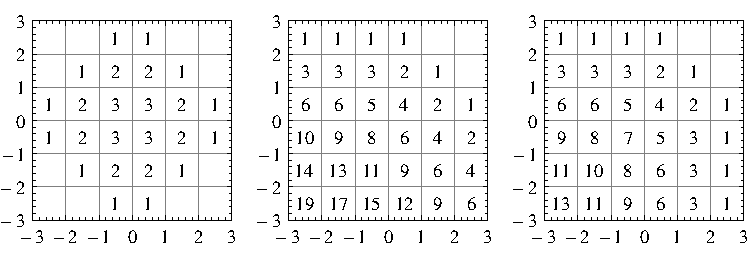
\includegraphics[width=130mm]{figures/irrep-verma-pverma.pdf}$
\end{lstlisting}

As we already stated properties of the module are encoded by its singular element. Function \lstinline{singularElement[m_module]} returns singular element of module as \lstinline{formalElement} datastructure. Character (up to \lstinline{limit} for (parabolic) Verma modules) is returned by function \lstinline{character[m_module]}. Direct sum of modules is module and we use natural notation
\begin{lstlisting}[mathescape=true]
im1=makeIrreducibleModule[$B_{2}$][weight[$B_{2}$][2,1]];
im2=makeIrreducibleModule[$B_{2}$][weight[$B_{2}$][1,2]];
textPlot[im1$\oplus$ im2]
$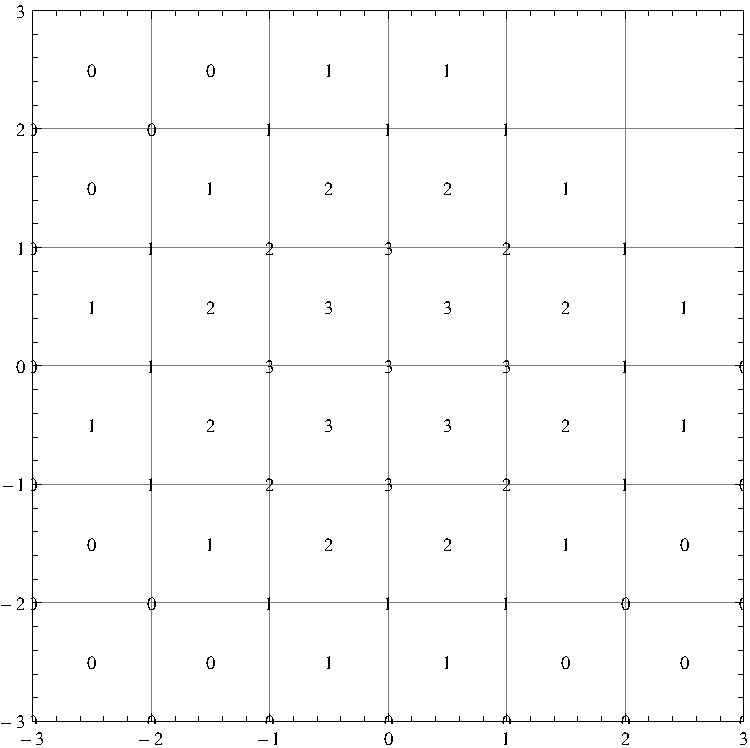
\includegraphics[width=60mm]{figures/irrep-sum.pdf}$
\end{lstlisting}

Tensor product is also implemented but only for finite-dimensional Lie algebras, since tensor product of affine Lie algebra modules leads to rich new structures \cite{kazhdan1994tensor3,kazhdan1993tensor1,kazhdan1993tensor2} which are out of the scope of present paper.

\section{Computational algorithms}
\label{sec:comp-algor}

As we have already stated in section \ref{sec:high-weight-modul} there exist two recurrent relations which can be used to calculate weight multiplicities in irreducible modules. Both algorithms proceed in the following way to calculate weight multiplicities:
\begin{enumerate}
\item Create the list of weights in main Weyl chamber by subtraction of all possible combinations of simple roots from the highest weight (e.g. for finite-dimensional algebra subtract $\alpha_{1}$ from $\mu$ while inside $\bar C$, then subtract $\alpha_{2}$ from all the weights already obtained etc).
\item Sort the list of weights by their product with Weyl vector.
\item Use a recurrent formula. If the weight required for recurrent computation is outside the main chamber use Weyl symmetry.
\end{enumerate}
The difference in performance of algorithms is in the number of previous values required to get the multiplicity of weight under consideration. For recurrent relation \eqref{eq:14} it is constant and equal to the number of elements in Weyl group (if we are far from the boundary of representation diagram). When Freudenthal formula \eqref{eq:15} is used number of previous values grows with the distance from the external border of representation. So Freudenthal formula is faster if the weight is close to the border or the rank of the algebra and the size of Weyl group is large \cite{moody1982fast}.
Note that Freudenthal formula is valid for irreducible modules only, so it can not be used to study (generalized) Verma modules.

We have made some experiments with our implementations of Freudenthal formula and formula \eqref{eq:15} and have got Figure  \ref{fig:freudenthal-racah-times}, which depicts dependence of computation time on number of weights in module.

\begin{figure}[h]
  \noindent\centering{
    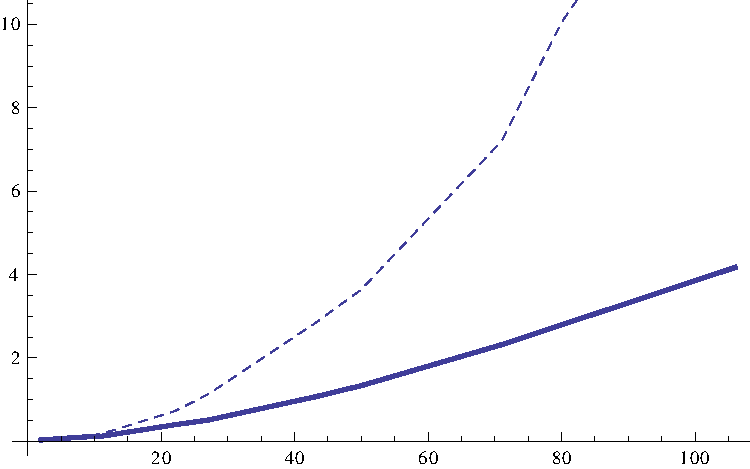
\includegraphics[width=80mm]{figures/timing.pdf}
  }
  \caption{Running time of algorithms based on recurrent formula \eqref{eq:15} (in blue) and \eqref{eq:14} (in red) with the number of weights in $\bar C$ for calculation of multiplicities in representations of $B_{2}$.}
\label{fig:freudenthal-racah-times}

\end{figure}

In the calculation of branching coefficients use of Freudenthal formula requires full construction of formal characters of algebra representation and all the representations of subalgebra. It is impractical when the rank of algebra and subalgebra are big, for example for maximal subalgebra.

Alternative algorithm which was presented in the paper \cite{2010arXiv1007.0318L} proceeds as follows:
It contains the following steps:

\begin{enumerate}
\item  Construct the root system $\Delta _{\af}$ for the embedding $%
\af\rightarrow \frak{g}$.

\item  Select all positive roots $\alpha \in \Delta ^{+}$ orthogonal
to  $\af$, i.e. form the set $\Delta_{\afb }^{+}$.

\item  Construct the set $\Gamma _{\af\rightarrow \frak{g}}$. Relation
 (\ref{eq:6}) defines the sign function
 $s(\gamma)$ and the set $\Phi_{\af\subset \frak{g}}$ where the lowest weight
 $\gamma_0$ is to be subtracted to get the fan:
 $\Gamma _{\af\rightarrow \frak{g}}=\left\{ \xi -\gamma _{0}|\xi \in \Phi _{%
\af\subset \frak{g}}\right\} \setminus \left\{ 0\right\}$.

\item  Construct the set $\widehat{\Psi ^{(\mu )}}=\left\{ w (\mu +\rho
)-\rho ;\;w \in W\right\} $ of singular weights for the $\frak{g}$%
-module $L^{(\mu )}$.

\item  Select the weights $\left\{ \mu _{\widetilde{\af_{\perp }}%
}\left( w\right) =\pi _{\widetilde{\af_{\perp }}}\left[ w(\mu +\rho
)-\rho \right] -\mathcal{D}_{\af_{\perp }}\in \overline{C_{\widetilde{%
\af_{\perp }}}}\right\} $. Since the set $\Delta_{\afb }^{+}$ is fixed
we can easily check wether the weight $\mu _{\widetilde{\af_{\perp }}%
}\left( w\right) $ belongs to the main Weyl chamber $\overline{C_{\widetilde{%
\af_{\perp }}}}$ (by computing its scalar product with the fundamental
weights of $\afb^{+}$).

\item  For the weights $\mu _{\widetilde{\af_{\perp }}}\left( w\right) $
calculate dimensions of the corresponding modules, $\mathrm{\dim }\left(
L_{\widetilde{\af_{\perp }}}^{\mu _{\widetilde{\af_{\perp }}%
}\left( u\right) }\right) $, using the Weyl dimension formula and construct
the singular element $\Psi ^{\left( \mu \right) }_{\left(  \af, \afb \right)}$.

\item  Calculate the anomalous branching coefficients using the
recurrent relation (\ref{recurrent-rel}) and select among them those
corresponding to the weights in the main Weyl
chamber $\overline{C_{\af}}$.
\end{enumerate}

We can speed up the algorithm by
one-time computation of the representatives of the conjugate classes $%
W/W_{\afb }$.


Consider the regular embedding $B_{2}\subset B_{4}$. In this case fan consists of 24 elements. In order to decompose $B_{4}$ module we need to construct the subset of singular weights of the module which projects to the main Weyl chamber of subalgebra $B_{2}$. Full set of singular weights consists of 384 elements. Required subset contains at most 48 elements. So time of the construction of required subset is negligible if the number of branching coefficients is greater than that. We may estimate the total number of required operations for the computation of branching coefficients as the product of number of elements in main Weyl chamber of subalgebra with non-zero branching coefficients and number of elements in fan. In the case of direct algorithm we need to compute the multiplicities for each module in the decomposition, so the number of operations grows faster than square of number of elements in main Weyl chamber of subalgebra with non-zero branching coefficients. 

To further illustrate this performance issue we include the Figure \ref{fig:branching} where we show the time required for computations of branching coefficients for $B_{3}\subset B_{4}$.

\begin{figure}[h]
  \noindent\centering{
   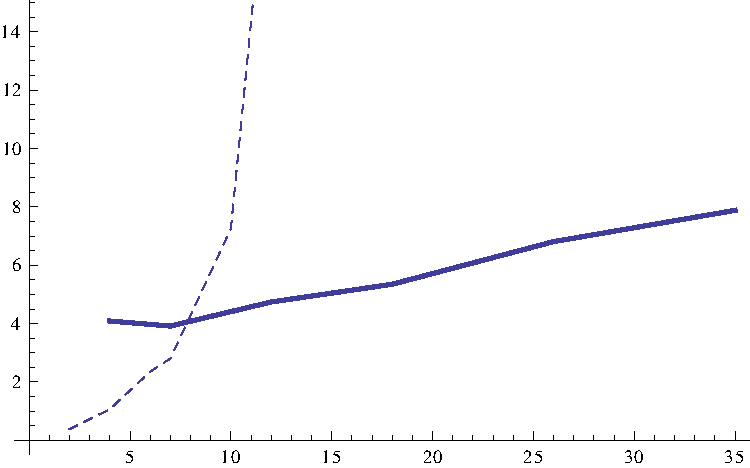
\includegraphics[width=100mm]{figures/branching-timing.pdf}
  }
  \caption{Running time of algorithms based on recurrent formula \eqref{eq:15} (in blue) and \eqref{eq:14} (in red) with the number of weights in $\bar C$ for calculation of branching coefficients for $B_{3}\subset B_{4}$.}
  \label{fig:branching}
\end{figure}

\section{Examples}
\label{sec:examples}
In this section we present some examples of computations available with {\bf Affine.m} with the code required to produce these results.

\subsection{Tensor product decompositon for finite-dimensional Lie algebras}
\label{sec:tens-prod-decomp}

Computation of fusion coefficients for the decomposition of tensor product of highest-weight modules to the direct sum of irreducible modules has numerous applications in physics. For example, we can consider spin of composite system such as atom. Another interesting example is integrable spin chain consisting of $N$ particles with the spins living in some representation $L$ of Lie algebra $\gf$ with $\gf$-invariant Hamiltonian $H$, describing nearest-neighbour spin-spin interaction. In order to solve such system, i.e. find eigenstates of Hamiltonian, we need to decompose $L^{\otimes N}$ into the direct sum of irreducible $\gf$-modules of lower dimension and diagonalize the Hamiltonian on these modules.

For fundamental representations of simple Lie algebras it is sometimes possible to get analytic result for the dependence of decomposition coefficients on $N$ (See \cite{LyakhovskyPostnova2011}). Our code give numerical values and can be used to check this analytic results.

Consider tensor power of $B_{2}$ first fundamental representations $\left(L^{[1,0]}\right)^{\otimes 4}$. Decomposition coefficients are just branching coefficients for tensor product module to the diagonal subalgebra $B_{2}\subset B_{2}\oplus B_{2}\oplus B_{2}\oplus B_{2}$. So following code calculates these coefficients:
\begin{lstlisting}[mathescape=true]
fm = makeIrreducibleModule[$B_{2}$][1, 0];
tp = ((fm$\otimes$ ]fm)$\otimes$ fm)$\otimes$]fm;
subs = makeFiniteRootSystem[
  {1/4*{1, -1, 1, -1, 1, -1, 1, -1}, 
   1/4*{0, 1, 0, 1, 0, 1, 0, 1}}];
bc = branching[tp, subs];
{bc[#], dynkinLabels[subs][#]} & /@ bc[weights]
\end{lstlisting}
It produces list of highest weights and tensor product decomposition coefficients:
\begin{lstlisting}
{{1, {4, 0}}, {3, {2, 2}}, {0, {3, 0}}, 
{2, {0, 4}}, {3, {1, 2}}, {6, {2, 0}}, 
{6, {0, 2}}, {1, {1, 0}}, {3, {0, 0}}}]
\end{lstlisting}

Returning to the problem of spin chain Hamiltonian diagonalization we can see that instead of diagonalizing operator in space of dimension $625$ we can diagonalize operators in spaces of dimensions $55, 81, 30, 35, 35, 14, 10, 5, 1$.

\subsection{Branchig and parabolic Verma modules}
\label{sec:branch-parab-verma}

We illustrate generalized BGG-resolution with the diagrams of $G_{2}$ parabolic Verma modules which appear in the decomposition of irreducible module $L^{[1,1]}_{G_{2}}$:
\begin{equation}
\mathrm{ch}\left( L^{\mu }\right) =\sum_{u\in U}\;e^{\mu _{\aft}\left(
u\right) }\epsilon (u)\mathrm{ch}M_{I}^{\mu _{\frak{a}_{\perp }}\left(
u\right) }.  \label{char-in-gen-verma-mod}
\end{equation}
Character of $L^{[1,1]}$ is presented in Figure \ref{branching-bgg}, characters of generalized Verma modules in decomposition \eqref{char-in-gen-verma-mod} are shown in Figure \ref{g2-pverma}. Characters in upper row appear in \eqref{char-in-gen-verma-mod} with positive sign and in lower row with negative.


\begin{figure}[h]
  \noindent\centering{
    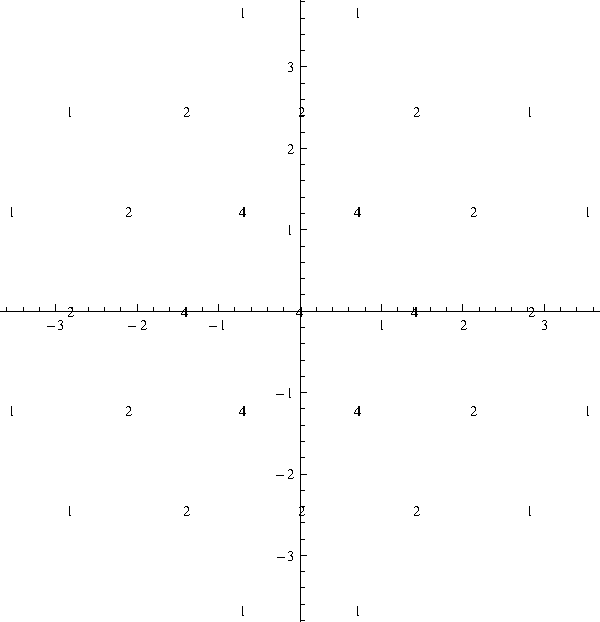
\includegraphics[width=80mm]{figures/G2-irrep.pdf}
  }
  \caption{Character of irreducible $G_{2}$-module $L^{[1,1]}$}
  \label{branching-bgg}
\end{figure}
\begin{figure}[h]
  \noindent\centering{
    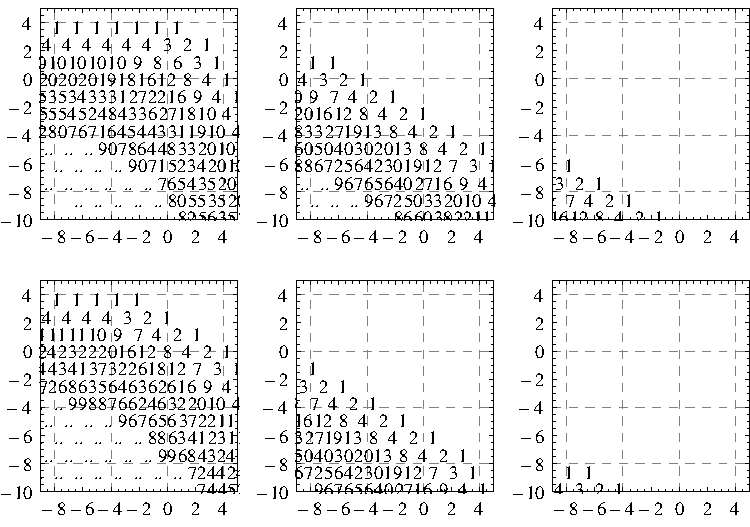
\includegraphics[width=150mm]{figures/G2-pverma.pdf}
  }
  \caption{Character of $G_{2}$ generalized Verma modules appearing in decomposition of $L^{[1,1]}$}
  \label{g2-pverma}
\end{figure}

\subsection{String functions of affine Lie algebras and CFT models}
\label{sec:string-funct-affine}

String functions can be used to present the formal character of affine Lie algebra highest weight representation. They have interesting analytic and modular properties \cite{kac1990idl,kac1988modular,kac1984infinite}.

String functions can be given physical meaning if we consider coset models of two-dimensional conformal field theory \cite{Goddard198588}, \cite{difrancesco1997cft}. String functions of $\hat\gf$ are equal to branching functions in the case of subalgebra $\hat{u(1)}$ and can be seen as the partition functions of $\hat\gf/\hat{u(1)}$ coset model on the torus.

{\bf Affine.m} produces power series decomposition for string functions. Consider affine Lie algebra $\hat{sl(3)}=\hat A_{2}$ highest weight module $L^{(1,0,0)}$. To get string functions we can use the code:
\begin{lstlisting}[mathescape=true]
stringFunctions[$\hat A_2$,{1,1,2}]
{{0, 0, 4}, 
  $2 q + 10 q^2 + 40 q^3 + 133 q^4 + 398 q^5 + 1084 q^6 + 2760 q^7 + 6632 q^8 + 15214 q^9 + 33508 q^{10}$}, 
{{0, 3, 1}, 
  $2 q + 12 q^2 + 49 q^3 + 166 q^4 + 494 q^5 + 1340 q^6 + 3387 q^7 + 8086 q^8 + 18415 q^9 + 40302 q^{10}$}, 
{{1, 1, 2}, 
  $1 + 6 q + 27 q^2 + 96 q^3 + 298 q^4 + 836 q^5 + 2173 q^6 + 5310 q^7 + 12341 q^8 + 27486 q^9 + 59029 q^{10}$}, 
{{2, 2, 0}, 
  $1 + 8 q + 35 q^2 + 124 q^3 + 379 q^4 + 1052 q^5 + 2700 q^6 + 6536 q^7 + 15047 q^8 + 33248 q^9 + 70877 q^{10}$}, 
{{3, 0, 1}, 
  $2 + 12 q + 49 q^2 + 166 q^3 + 494 q^4 + 1340 q^5 + 3387 q^6 + 8086 q^7 + 18415 q^8 + 40302 q^9 + 85226 q^{10}$}
\end{lstlisting}

\subsection{Branching functions and coset models of conformal field theory}
\label{sec:branch-funct-coset}

More complex models of CFT can be obtained from cosets $G/A$ corresponding to the embedding $\af\subset\gf$. These models can be studied as gauge theories \cite{Hwang:1994yr, hwang1993brst}.

Branching functions of the embedding $\af\subset\gf$ are the partition functions of CFT on the torus (see \cite{difrancesco1997cft}).

As first example we show computation of branching functions for the embedding $\hat A_{1}\to \hat B_{2}$ up to tenth grade:
\begin{lstlisting}[mathescape=true]
branchingFunctions[$\hat B_{2}$,makeAffineExtension[makeFiniteRootSystem[{{1, 1}}]], {1, 1, 1}]

 {{3, 0}, 
  $2 + 14 q + 52 q^2 + 154 q^3 + 410 q^4 + 994 q^5 + 2248 q^6 + 4832 q^7 + 9934 q^8 + 19680 q^9 + 37802 q^{10}$},
 {{2, 1}, 
  $4 + 20 q + 72 q^2 + 220 q^3 + 584 q^4 + 1424 q^5 + 3248 q^6 + 7012 q^7 + 14488 q^8 + 28844 q^9 + 55616 q^{10}$},
 {{0, 3}, 
  $4 q + 20 q^2 + 68 q^3 + 200 q^4 + 516 q^5 + 1224 q^6 + 2736 q^7 + 5808 q^8 + 11820 q^9 + 23236 q^{10}$},
 {{1, 2}, 
  $2 + 14 q + 54 q^2 + 168 q^3 + 462 q^4 + 1148 q^5 + 2656 q^6 + 5812 q^7 + 12130 q^8 + 24358 q^9 + 47328 q^{10}$}
\end{lstlisting}

Another example is computation of branching functions for the regular embedding $\hat B_{2}\subset \hat C_{3}$:
\begin{lstlisting}[mathescape=true]
sub=makeAffineExtension[parabolicSubalgebra[$C_{3}$][2,3]];
branchingFunctions[$\hat C_{3}$,sub, {2, 0, 0, 0}]

{{0, 1, 0}, 
  $2 q - 20 q^3 + 24 q^4 + 82 q^5 - 320 q^6 + 108 q^7$}, 
{{1, 0, 0}, 
  $1 - q - 8 q^2 + 19 q^3 + 16 q^4 - 156 q^5 + 205 q^6 + 640 q^7$}, 
{{0, 0, 1}, 
  $q - 5 q^3 + 7 q^5$}
\end{lstlisting}

\section{Conclusion}
\label{sec:conclusion}
We have presented the package {\bf Affine.m} for computations in representation theory of finite-dimensional and affine Lie algebras. It can be used to study Weyl groups, roots systems, irreducible, Verma and parabolic Verma modules of finite-dimensional and affine Lie algebras.  In present paper we have also discussed main ideas used for implementation of the package and described most important notions of representation theory required to use {\bf Affine.m}. 

We have demonstrated that recurrent approach based upon Weyl character formula is not only useful for calculations but also allows to see connection with (generalized) Bernstein-Bernstein-Gelfand resolution. 

Also we have presented examples of computations with this package connected with problems of physics and mathematics. 

\section*{Acknowledgements}
\label{sec:acknowledgements}
The work is supported by the Chebyshev Laboratory
(Department of Mathematics and Mechanics, Saint-Petersburg State
University) under the grant 11.G34.31.0026 of the Government of the
Russian Federation.


%% The Appendices part is started with the command \appendix;
%% appendix sections are then done as normal sections
\appendix

\section{Software package}
\label{package}
The package can be freely downloaded from \url{http://github.com/naa/Affine}. To get the development code use the command
\begin{lstlisting}[language=bash]
 git clone git://github.com/naa/Affine.git
\end{lstlisting}

Contents of the package:
\begin{verbatim}
    Affine/                                root folder
      demo/                                  demonstrations
        demo.nb                                demo notebook
        paper.nb                               code for the paper
      doc/                                 documentation folder
        figures/                             figures in paper 
          timing.pdf                           diagram showing performance
          branching-timing.pdf                 ...  for branching coefficients  
          irrep-sum.pdf                        sum of B2 irreps
          irrep-verma-pverma.pdf               irrep, Verma, (p)Verma for B2
          G2-irrep.pdf                         irrep for G2
          G2-pverma.pdf                        parabolic Verma for G2
        bibliography.bib                     bibliographic database
        paper.pdf                            present paper
        paper.tex                            paper source
        TODO.org                             list of issues
      src/                                 source folder
        affine.m                             main software package
      tests/                               unit tests folder
        tests.m                              unit tests
      README.markdown                      installation and usage notes
\end{verbatim}


%% References
%%
%% Following citation commands can be used in the body text:
%% Usage of \cite is as follows:
%%   \cite{key}         ==>>  [#]
%%   \cite[chap. 2]{key} ==>> [#, chap. 2]
%%

%% References with bibTeX database:

\section*{References}
\label{sec:references}


\bibliography{bibliography}
\bibliographystyle{elsarticle-num}
%\bibliographystyle{model1-num-names}


%% Authors are advised to submit their bibtex database files. They are
%% requested to list a bibtex style file in the manuscript if they do
%% not want to use elsarticle-num.bst.

%% References without bibTeX database:

% \begin{thebibliography}{00}

%% \bibitem must have the following form:
%%   \bibitem{key}...
%%

% \bibitem{}

% \end{thebibliography}


\end{document}

%%
%% End of file